\documentclass[12pt, a4paper]{report}

% --- Packages ---
\usepackage[utf8]{inputenc}
\usepackage[T1]{fontenc}
\usepackage[english]{babel}
\usepackage{geometry}
\geometry{a4paper, left=3cm, right=2.5cm, top=2.5cm, bottom=2.5cm}
\usepackage{graphicx}
\graphicspath{{./}}
\usepackage{setspace}
\setstretch{1.15} 
\usepackage{siunitx} % For proper SI unit formatting (e.g., \SI{20}{m})
\usepackage{hyperref}
\hypersetup{
    colorlinks=false,
    hidelinks
}
\usepackage[printonlyused]{acronym}
\usepackage{csquotes}

% --- IEEE Bibliography Setup ---
\usepackage[backend=biber, style=ieee]{biblatex}
\addbibresource{references.bib}

\begin{document}

% ==========================================
% 1. TITLE PAGE 
% ==========================================
\begin{titlepage}
    \noindent
    
\includegraphics[width=0.3\textwidth]{fh_logo.png}\par\vspace{3cm}
    
    \centering
    {\Huge\bfseries Semantic information extraction from a 3D point
cloud\par}
    \vspace{0.5cm}
    % {\Large\itshape (Migrating to GPU-Accelerated Sparse Transformers)\par}
    \vspace{3cm}
    
    {\Large \textbf{Project Work 1}\par}
    \vspace{0.3cm}
    {\large in the study program ``Master of Information Technology''\par}
    \vspace{2cm}
    
    submitted by\par
    \vspace{0.5cm}
    {\large \textbf{Aikaterini Papagiannitsi}\par}
    Matriculation Number: 7224598\par
    \vspace{1.5cm}
    
    on \today\par
    at Fachhochschule Dortmund\par

    
    \begin{flushleft}
        First Examiner: \par
        Second Examiner:
    \end{flushleft}
    \vfill
\end{titlepage}
\newpage
\thispagestyle{empty}
\mbox{}
\addtocounter{page}{-1}
\newpage

% ==========================================
% 2. ABSTRACT
% ==========================================
\begin{abstract}
This report details the methodology, testing, and validation of adapting a pretrained 3D semantic segmentation model (\ac{PTv3}) to out-of-domain, high-density static LiDAR point clouds. The model, originally trained on the automotive nuScenes dataset, exhibits strong domain shift when applied to data captured by an FJD Trion S1 scanner. A zero-shot adaptation pipeline is evaluated, combining spatial tiling, feature camouflage (intensity masking), and geometric downsampling that simulates 32-beam Velodyne-like ring structures. The report also documents environment setup challenges on modern hardware (NVIDIA RTX 5090) and the transition to a containerized, hardware-compatible inference stack. In the ablation study, the best configuration raises 4-class \ac{mIoU} from 5.29\% to 16.84\%.
\end{abstract}

% ==========================================
% 3. DIRECTORIES (TOC, Figures, Abbreviations)
% ==========================================
\tableofcontents
\newpage

\listoffigures
\addcontentsline{toc}{chapter}{List of Figures}
\newpage

\chapter*{List of Abbreviations}
\addcontentsline{toc}{chapter}{List of Abbreviations}
\begin{acronym}[SLAM] % The word in brackets sets the indentation width
    \acro{SLAM}{Simultaneous Localization and Mapping}
    \acro{CPU}{Central Processing Unit}
    \acro{GPU}{Graphics Processing Unit}
    \acro{PTv3}{Point Transformer V3}
    \acro{AI}{Artificial Intelligence}
    \acro{CNN}{Convolutional Neural Network}
    \acro{IoU}{Intersection over Union}
    \acro{mIoU}{mean Intersection over Union}
    \acro{UDA}{Unsupervised Domain Adaptation}
    \acro{LAS}{LAS point cloud format}
\end{acronym}
\newpage

% ==========================================
% 4. MAIN BODY
% ==========================================
% AI Transparency Declaration
\noindent\textit{\textbf{\ac{AI} Transparency Declaration:} In accordance with university guidelines, AI tools (specifically Google Gemini) were utilized to assist in structuring the English phrasing of this report. All factual claims, architectural decisions, and code implementations remain the original work of the author.}

\chapter{Motivation}
3D semantic segmentation is a key step for transforming raw point clouds into machine-interpretable urban representations. In the context of urban planning, this enables the creation and maintenance of Urban Digital Twins, where geometric structures are continuously enriched with semantic labels (e.g., ground, vegetation, built structures, and dynamic objects).

This project investigates whether a state-of-the-art automotive model can be reused for static terrestrial scans captured by an FJD Trion S1 LiDAR device. The practical motivation is to build a scalable and reproducible segmentation pipeline without immediate retraining, while still obtaining useful semantic outputs for downstream analysis.

\begin{figure}[h]
\centering
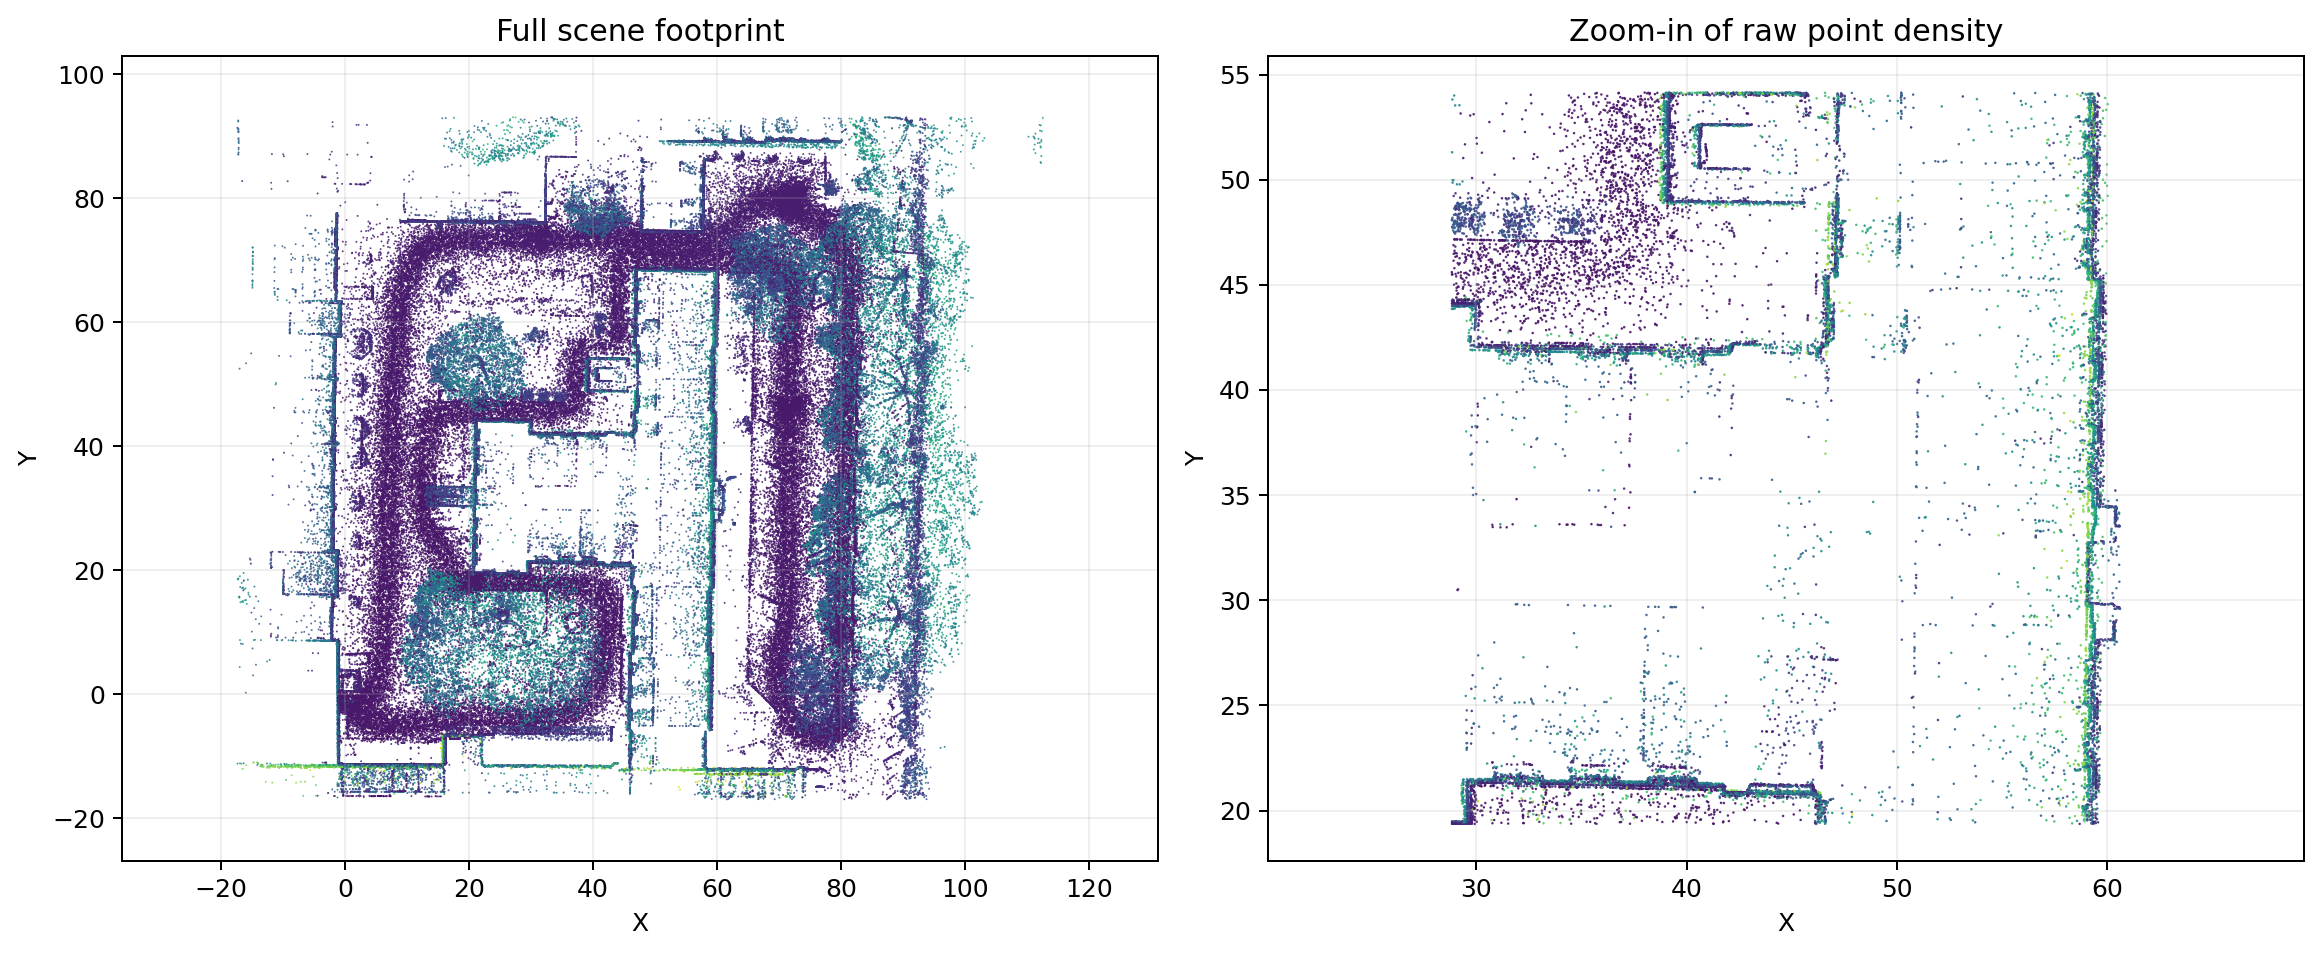
\includegraphics[width=0.9\textwidth]{figures/scene_overview.png}
\caption{Input scene overview used in this project (site context and raw point cloud).}
\label{fig:scene-overview}
\end{figure}


\chapter{Problem}
Two central problems are addressed in this work. First, dense urban point clouds are computationally expensive to process end-to-end due to high point counts and irregular spatial structure. Second, a big domain shift occurs when a model pretrained on nuScenes \cite{caesar2020nuscenes,nuscenes_website} is applied to FJD Trion S1 scans. In this report, domain shift refers to the mismatch between source and target data distributions, including sensor geometry, intensity calibration, viewpoint, and scene composition \cite{wang2020domain}.

Without adaptation, this mismatch causes large performance degradation and unstable class predictions. The project therefore focuses on zero-shot adaptation techniques that do not require immediate full-model retraining.

\section*{Research Questions}
The report is guided by three research questions:
\begin{enumerate}
    \item Can a nuScenes-pretrained \ac{PTv3} model generate useful semantic outputs on FJD Trion S1 scans without retraining?
    \item Which adaptation component contributes more to recovery under domain shift: intensity masking or ring-based geometric downsampling?
    \item Does remapping from 16 classes to 4 superclasses improve interpretability and stability for planning-oriented analysis?
\end{enumerate}

\section*{Evaluation Perspective}
Because this work targets zero-shot adaptation, success is assessed primarily by relative improvement over the direct baseline and by qualitative scene coherence. Absolute state-of-the-art performance on target-domain benchmarks is not expected without supervised fine-tuning.

\chapter{Literature Review}
The task of semantic segmentation in 3D point clouds involves assigning a categorical label to every individual point. Traditional deep learning approaches typically transform the unstructured 3D data into more manageable formats.

\begin{itemize}
    \item \textbf{Projection-based models} project the 3D points into 2D spherical or bird's-eye views, processing them with standard \acp{CNN}. While computationally efficient, these methods suffer from severe discretization errors and occlusion artifacts, losing critical 3D topology \cite{milioto2019rangenet}.

    \item \textbf{Voxel-based models} partition the space into 3D grids and apply sparse convolutions. Though highly accurate, they are heavily constrained by memory consumption when scaling to large outdoor environments \cite{choy20194d}.

    \item \textbf{Point-based models} process the raw points directly. Recent advancements have introduced transformer architectures to this domain. \ac{PTv3} \cite{wu2024ptv3} represents the state-of-the-art, overcoming previous computational bottlenecks by serializing point clouds and processing them with scaled dot-product attention, making it highly suitable for large-scale urban mapping.
\end{itemize}

Alongside architecture advances, domain adaptation has become a core challenge in LiDAR perception. Prior work shows that shifts in sensor design, acquisition viewpoint, and label distributions substantially degrade cross-domain performance \cite{wang2020domain}. In many practical projects, however, retraining is constrained by missing labels and limited compute budgets.

This report therefore focuses on a strict inference-time adaptation setting: no weight updates, no target labels, and no iterative pseudo-label training. The chosen strategy aligns target data with source-domain assumptions through deterministic preprocessing and semantic postprocessing. This makes the method operationally simple and reproducible while still yielding measurable gains.


\chapter{Methodology}
\section{Environment and GPU Acceleration}
To ensure reproducibility and isolate dependency conflicts, the processing environment was containerized with Podman, following standard reproducible-research practices for containerized workflows \cite{boettiger2015introduction}. Hardware acceleration was provided by an NVIDIA RTX 5090 \ac{GPU}. The final working stack used a CUDA 12.x compatible PyTorch build (PyTorch 2.7.0 with CUDA 12.8 support) to match the target hardware.

During environment setup, alternatives based on MinkowskiEngine were evaluated but were not reliable in this hardware and software combination. Therefore, the final implementation used Pointcept with \ac{PTv3} and a CUDA compatible sparse backend (spconv), enabling stable end-to-end inference.

From an engineering perspective, this setup was essential for two reasons. First, sparse 3D operators are highly sensitive to binary compatibility between CUDA, PyTorch, and compiled extensions. Second, the project required reproducibility across iterative experiments (baseline and adaptation variants), which is difficult to maintain in mutable local environments. Containerized execution ensured consistent dependencies for all ablation runs.


\section{Pipeline Overview}
The pipeline consists of three primary stages:
\begin{enumerate}
    \item \textbf{Tiling:} The raw FJD Trion S1 point cloud is first voxel-subsampled (\SI{0.05}{m}) and partitioned into overlapping \SI{30}{m} $\times$ \SI{30}{m} tiles with \SI{15}{m} stride.
    \item \textbf{Inference:} Each tile is processed independently by a pretrained \ac{PTv3} model. The nuScenes dataset \cite{caesar2020nuscenes,nuscenes_website} contains 32 semantic classes, but the \ac{PTv3} model used in this work was trained on a 16-class subset focusing on outdoor LiDAR-relevant categories.
    \item \textbf{Voting and Reconstruction:} Predictions from overlapping tiles are aggregated via softmax voting and then projected back to the original cloud geometry.
\end{enumerate}

Operationally, these stages map to three commands in the project workflow: tiling, inference, and reconstruction. This separation makes experiments easy to rerun with modified feature modes or geometric settings while keeping data preparation and output generation traceable.

\section{FJD Trion S1 vs. Automotive LiDAR}
A core challenge of this project is addressing the domain shift that occurs when a model pretrained on the automotive nuScenes dataset is applied to static FJD Trion S1 scans. The nuScenes data typically relies on a 32-beam Velodyne-like ring structure. By contrast, the FJD Trion S1 produces extremely dense geometry. Because of this discrepancy, direct application of the PTv3 model results in unstable class predictions, necessitating a zero-shot adaptation pipeline.

\section{Data Preprocessing and Tiling}
To accommodate \ac{GPU} memory constraints and preserve local geometry, the input \ac{LAS} file is partitioned into overlapping blocks. The point cloud is divided into \SI{30}{m} $\times$ \SI{30}{m} tiles using a \SI{15}{m} stride, resulting in a 50\% spatial overlap. A \SI{0.05}{m} voxel grid subsampling is applied within these tiles. This reduces the overall data density and computational load while maintaining the structural integrity of the urban environment.

In implementation terms, each tile stores local coordinates and metadata (global shift and indices to original points). This metadata is required for exact projection of predictions back to the original cloud during reconstruction. Overlap is deliberately retained to reduce edge artifacts and improve label consistency near tile boundaries.

\begin{figure}[h]
\centering
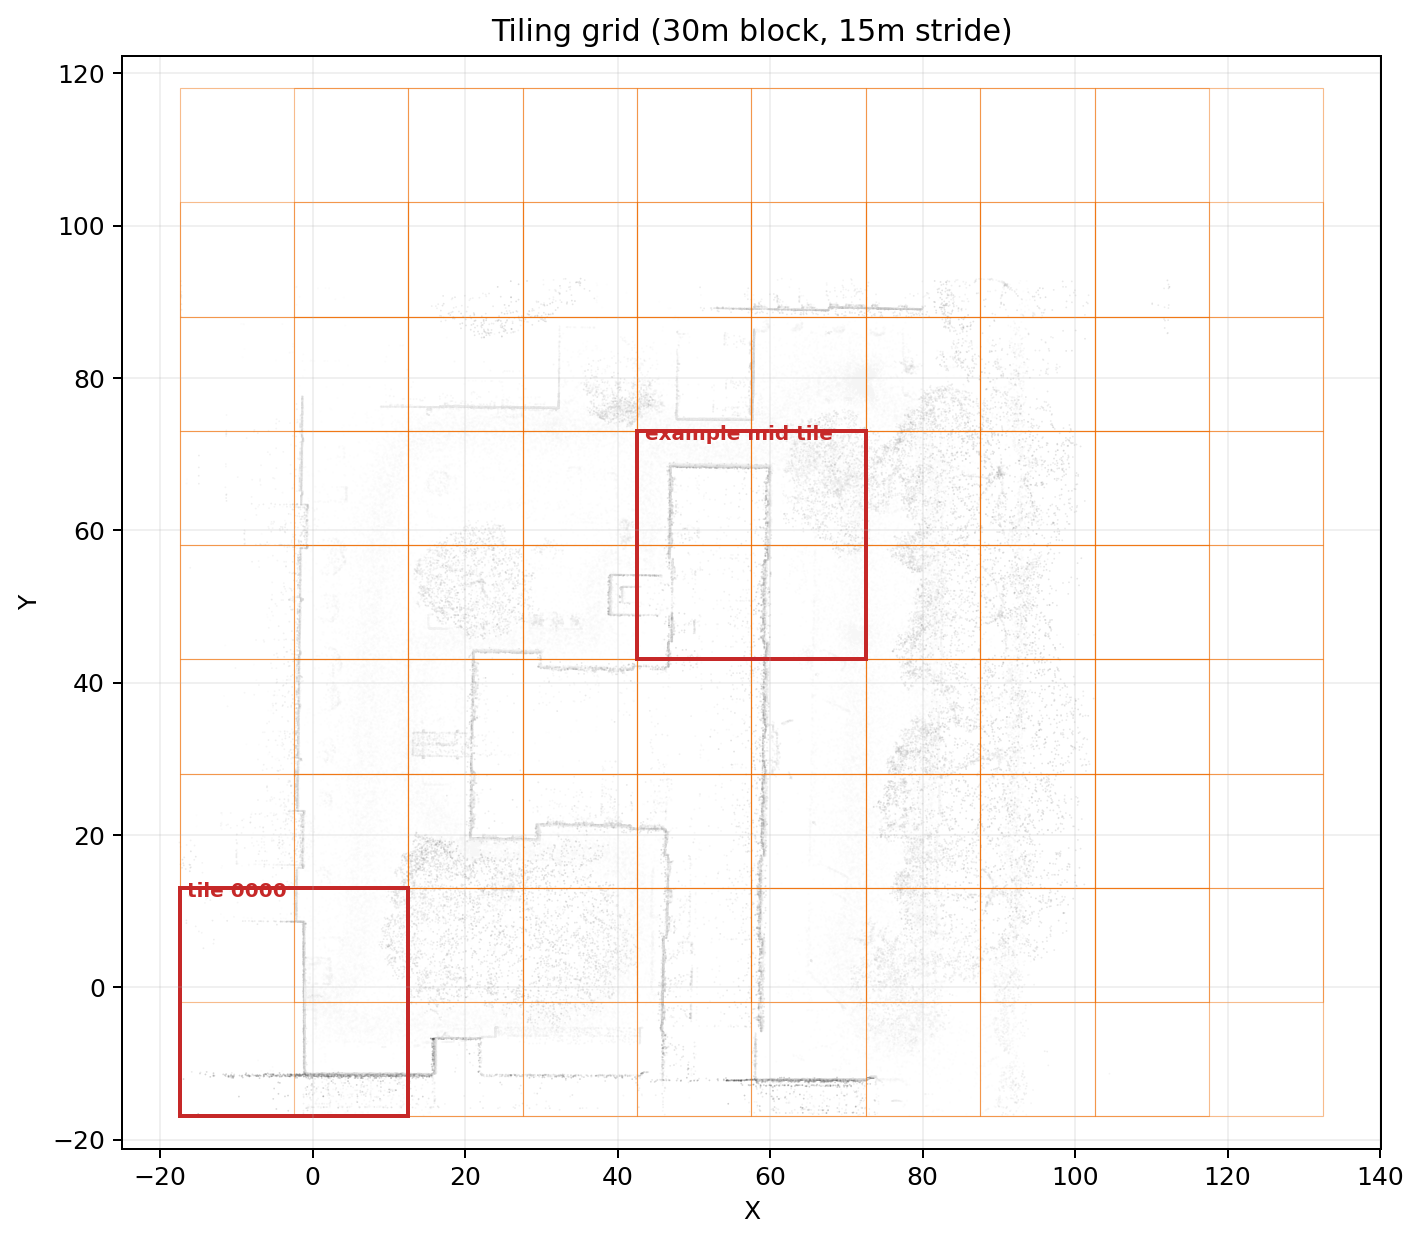
\includegraphics[width=0.9\textwidth]{figures/tiling_grid.png}
\caption{Spatial tiling strategy on the full scene (\SI{30}{m} $\times$ \SI{30}{m} windows, \SI{15}{m} stride).}
\label{fig:tiling-grid}
\end{figure}

\section{Domain Adaptation Strategies}
Inference is performed per tile using the pretrained \ac{PTv3} model. The core contribution is a zero-shot adaptation pipeline with three components:

\begin{enumerate}
    \item \textbf{Feature camouflage (zeroed intensity):} The nuScenes-pretrained model expects sensor-specific intensity statistics. To reduce misleading correlations, intensity is set to zero (\texttt{FEATURE\_MODE=zero}), forcing the model to rely on geometric features.
    \item \textbf{Geometric downsampling (Velodyne simulation):} FJD Trion S1 scans are much denser than automotive 32-beam LiDAR data. Points are transformed to spherical coordinates and filtered to mimic ring-like elevation structure. Two tolerances are evaluated: \SI{0.15}{\degree} (thick rings) and \SI{0.03}{\degree} (thin rings).
    \item \textbf{Semantic simplification:} Fine-grained automotive labels are remapped to broader classes relevant to urban planning.
\end{enumerate}

\begin{figure}[h]
\centering
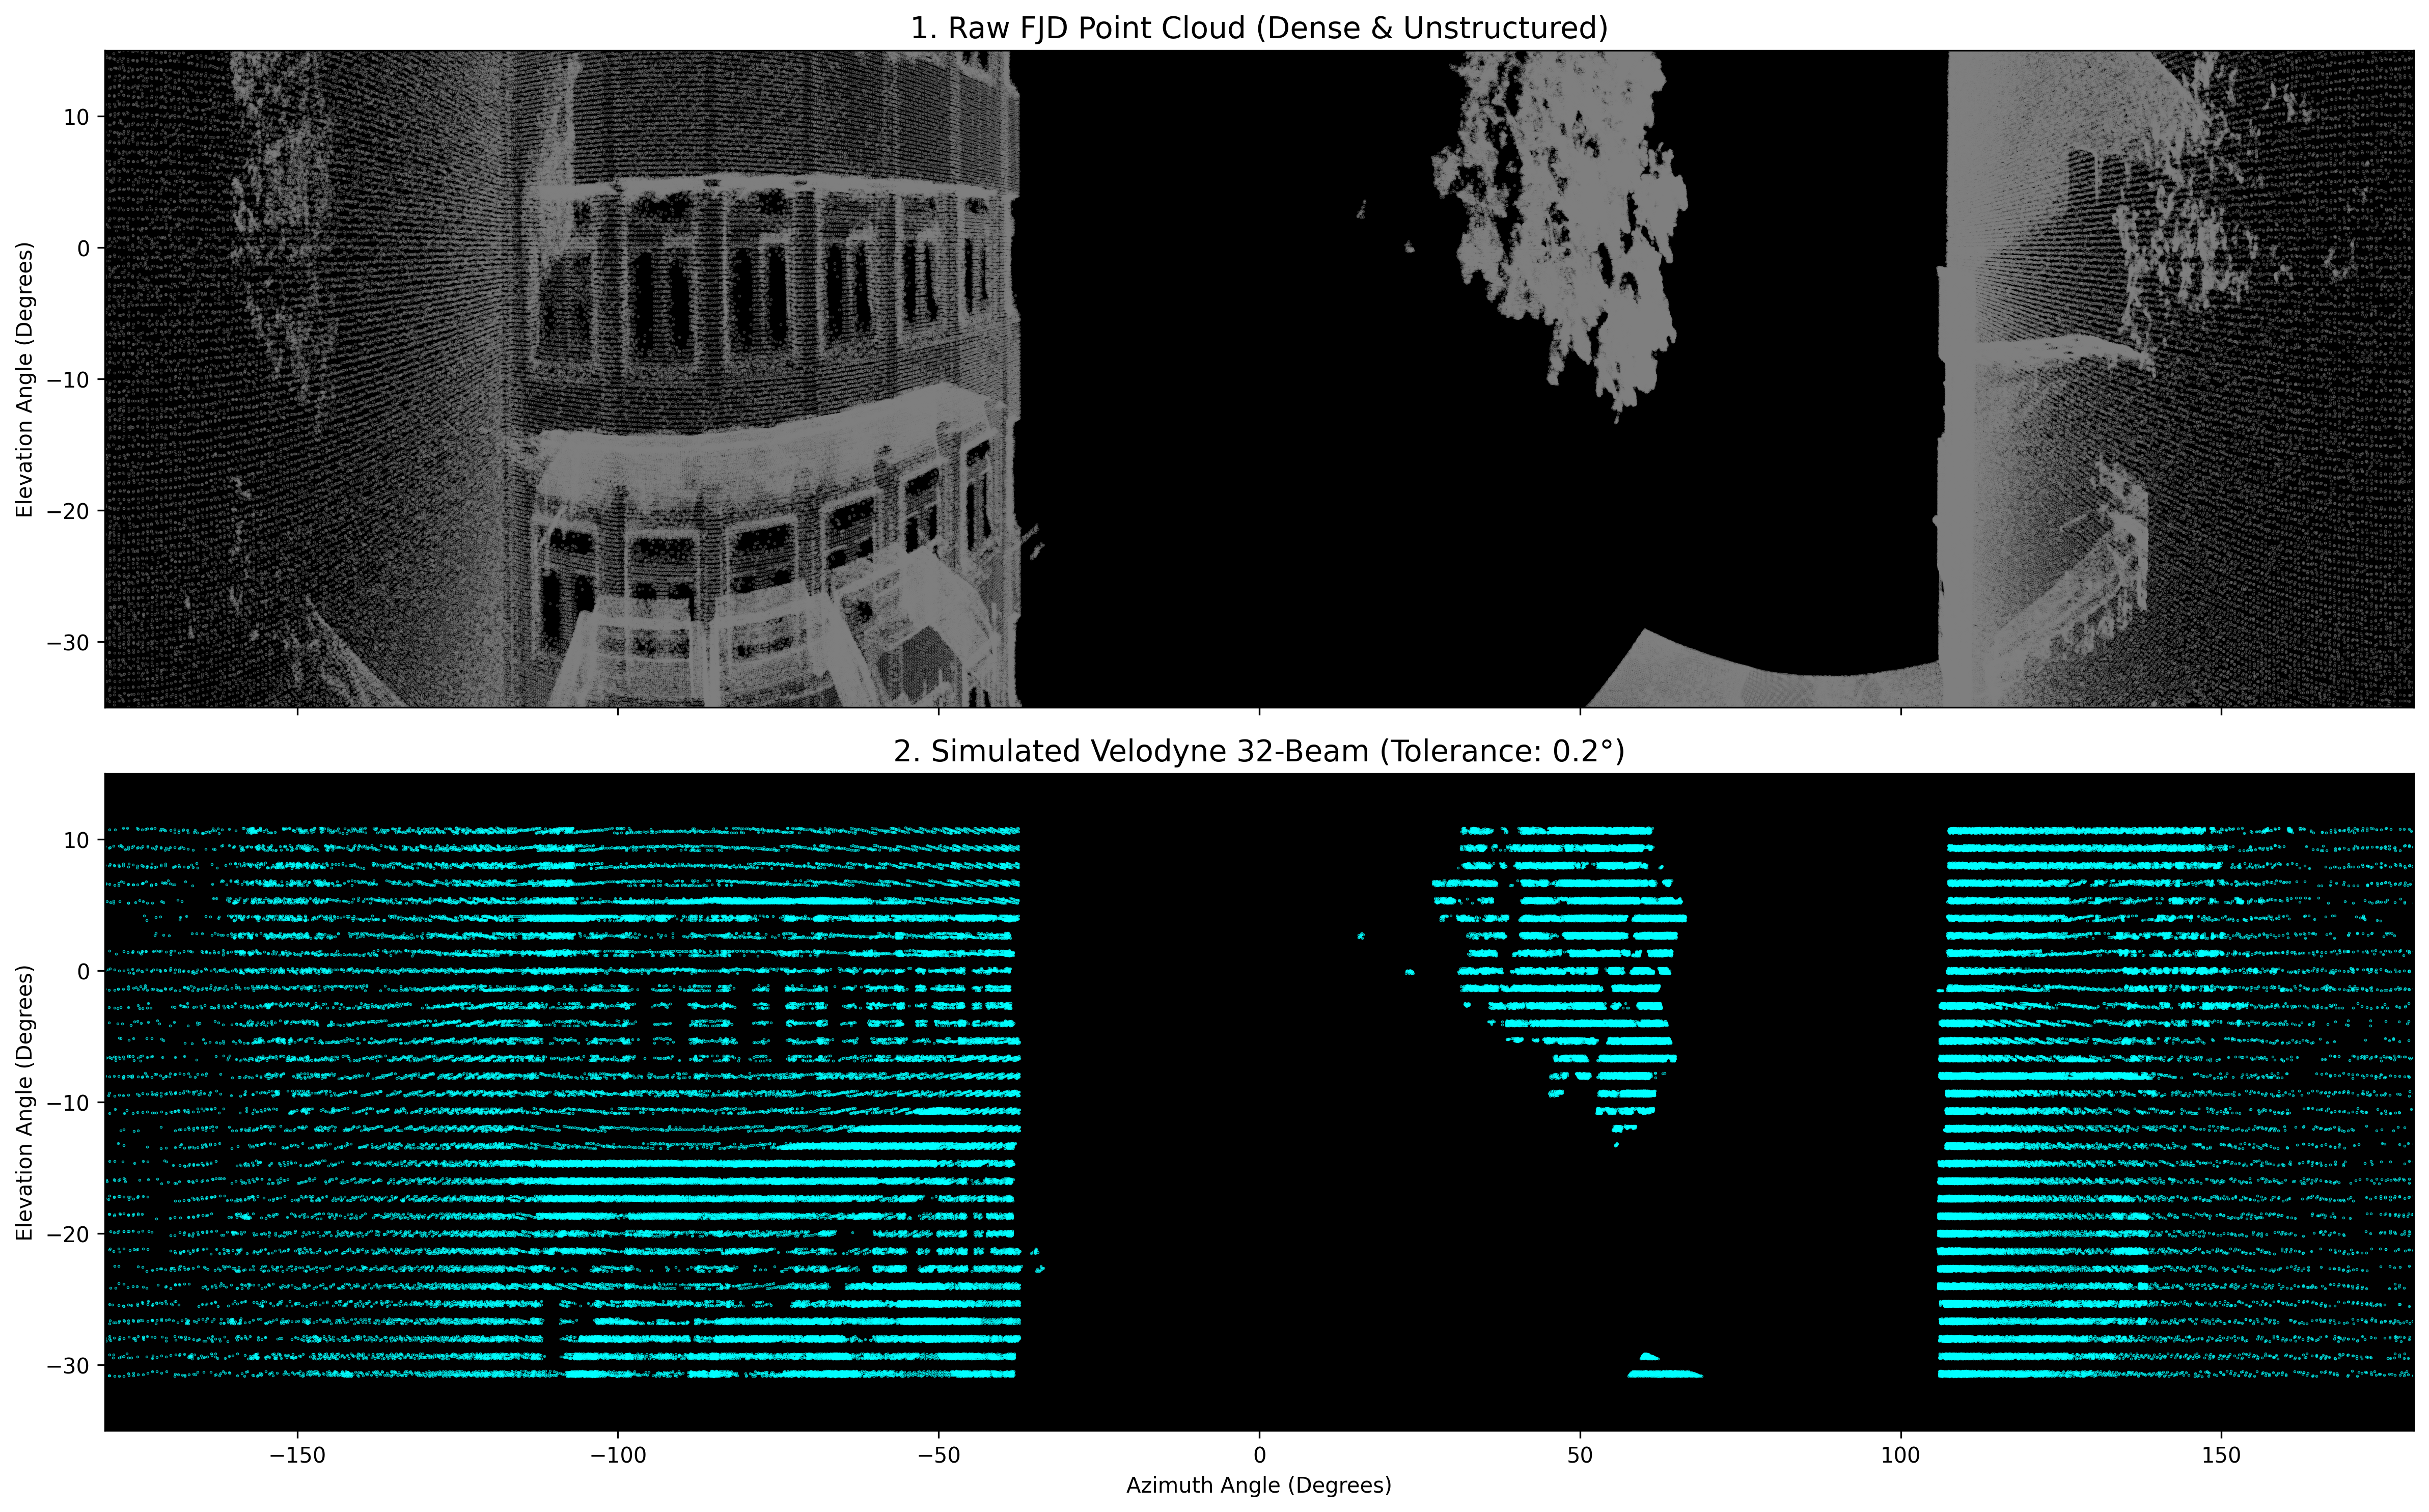
\includegraphics[width=0.9\textwidth]{ring_visualization.png}
\caption{Ring-structure simulation used for geometric domain adaptation.}
\label{fig:ring-simulation}
\end{figure}

\section{Target Space Mapping}
The \ac{PTv3} model outputs predictions across 16 classes derived from the nuScenes taxonomy. While the full nuScenes dataset defines 32 semantic classes, the pretrained model focuses on the 16 most common outdoor categories, excluding rare or indoor-specific labels. For the target use case, these 16 predictions are further remapped into four superclasses: \textit{Vegetation}, \textit{Object}, \textit{Ground}, and \textit{Structure}. This post-processing step reduces class noise and improves interpretability for planning-oriented analysis. The explicit class mapping is listed in Appendix~\ref{app:class-mapping}.

\begin{figure}[h]
\centering
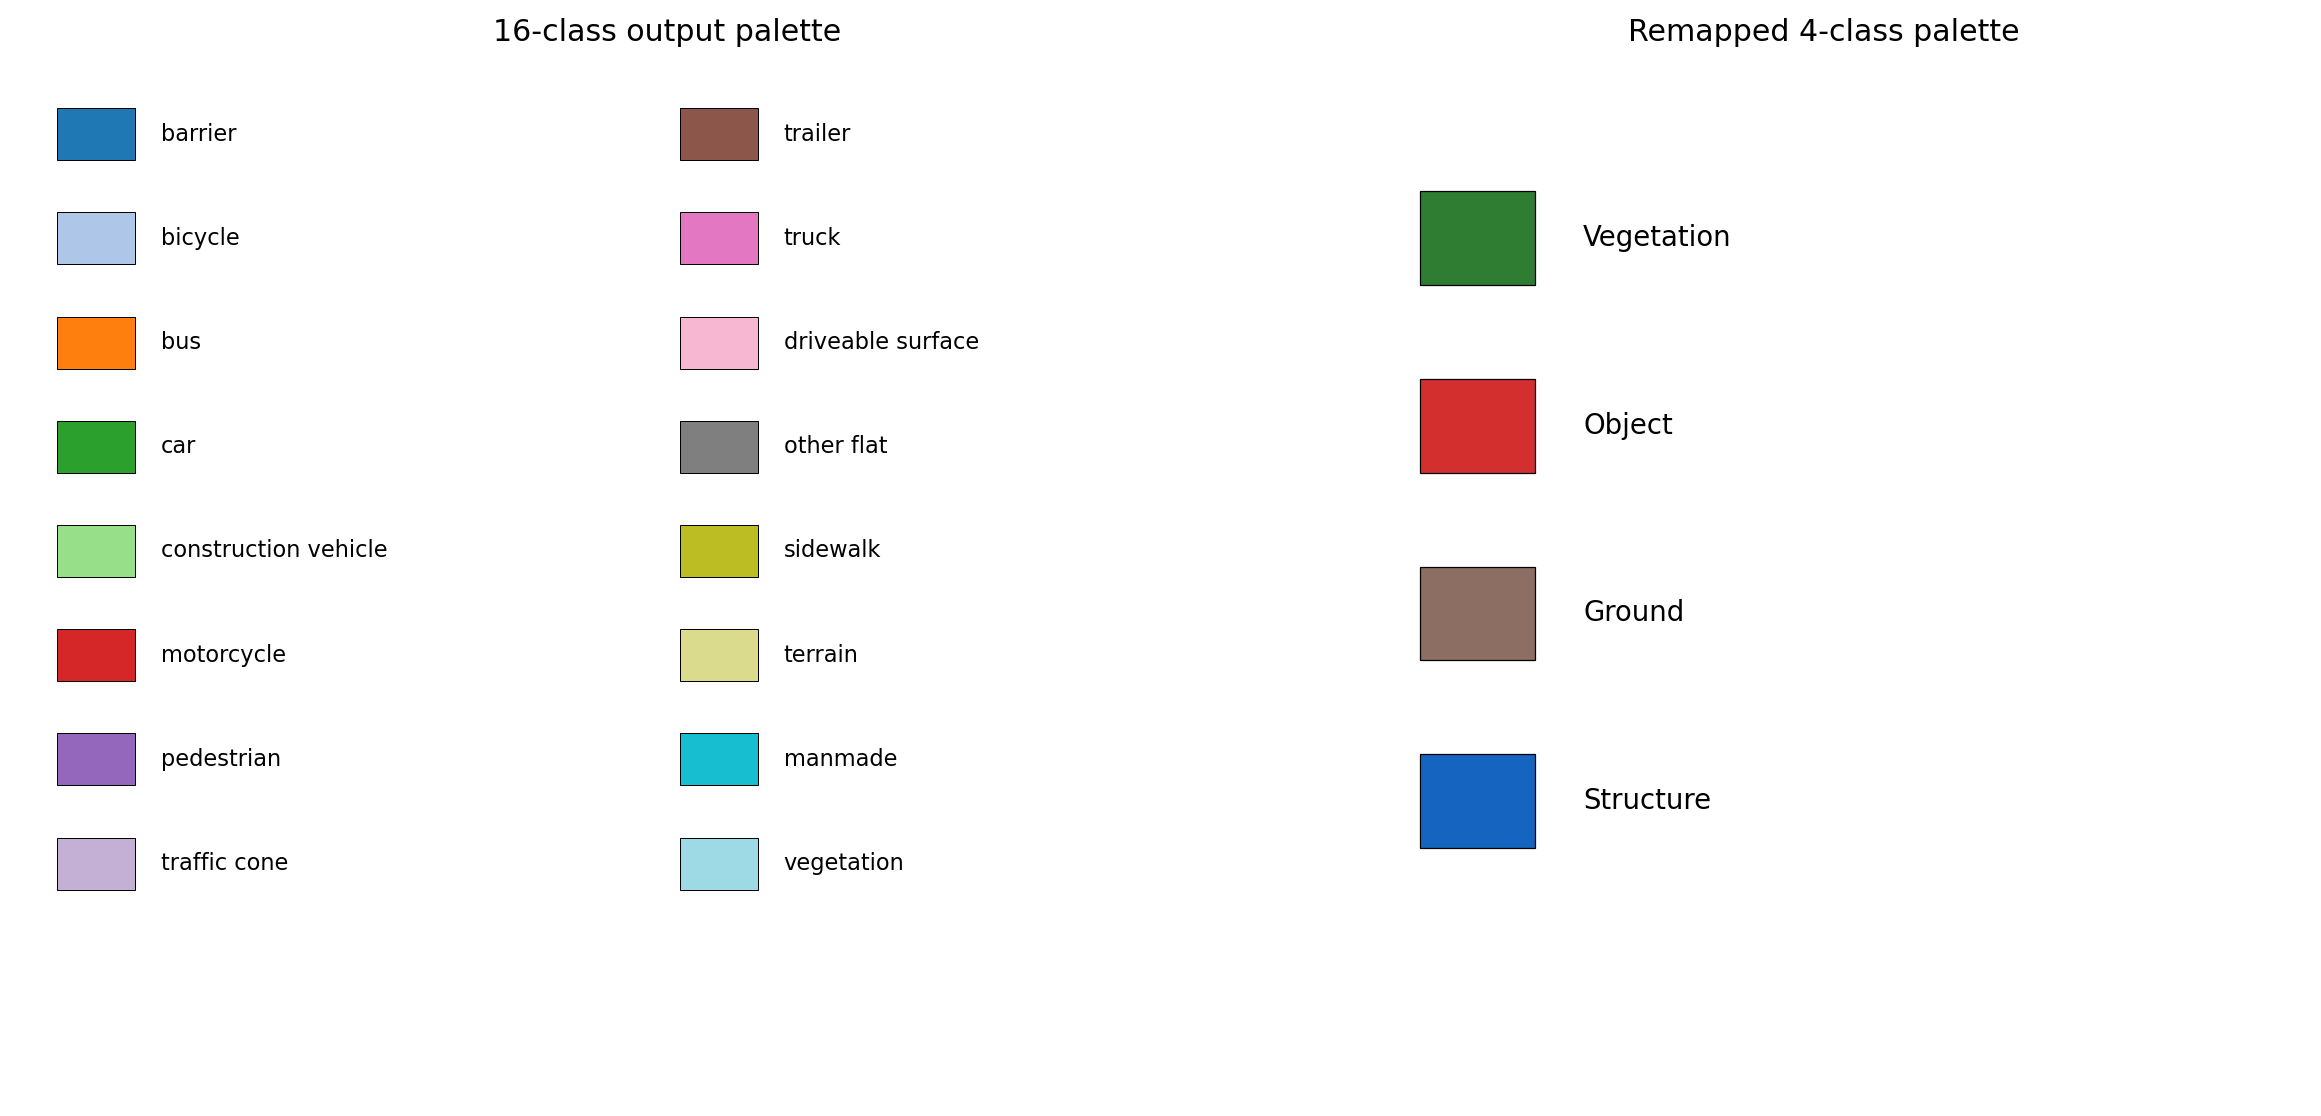
\includegraphics[width=0.9\textwidth]{figures/class_legend.png}
\caption{Visualization legend for original 16 classes and remapped 4-class superclasses.}
\label{fig:class-legend}
\end{figure}

\section{Reconstruction}
Following inference, the overlapping tiles must be reassembled. To handle the overlapping regions, the pipeline sums the output logits for points that exist in multiple tiles. A softmax function is then applied, and majority voting determines the final semantic label for each point. The consistently labeled point cloud is subsequently written back into a single \texttt{.las} file.

Two outputs are retained in the project workflow: one file with original 16-class predictions and one with the remapped 4-class predictions. Keeping both allows detailed error analysis in the source label space while providing a cleaner semantic view for application-oriented visualization.

\section{Implementation Workflow and Reproducibility}
For reproducibility, all experiments follow the same high-level command sequence:
\begin{enumerate}
    \item \texttt{make tile} (creates overlapping, voxelized tiles)
    \item \texttt{make infer FEATURE\_MODE=<mode>} (runs \ac{PTv3} on each tile)
    \item \texttt{make reconstruct} (aggregates overlapping predictions)
\end{enumerate}

The key controlled variables in this report are \texttt{FEATURE\_MODE} and ring tolerance. This design keeps model weights and reconstruction logic fixed, so measured differences can be attributed to adaptation choices rather than unrelated implementation changes.

\begin{figure}[h]
\centering
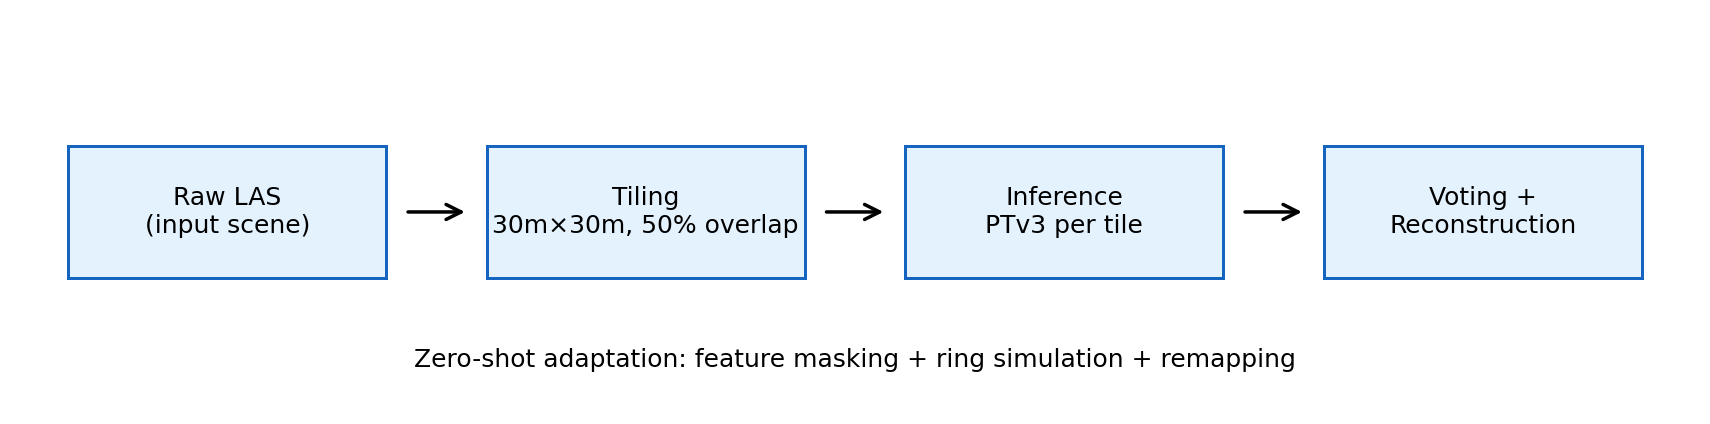
\includegraphics[width=0.9\textwidth]{figures/method_pipeline.png}
\caption{Processing pipeline used for zero-shot adaptation and semantic reconstruction.}
\label{fig:method-pipeline}
\end{figure}

\chapter{Test and Validation}
\section{Ablation Study Design}
An ablation study isolates the contribution of each adaptation component by changing one factor at a time while keeping the rest fixed. Four configurations were evaluated:

\begin{enumerate}
    \item \textbf{Config 1 (Baseline):} raw dense geometry with native FJD intensity.
    \item \textbf{Config 2:} raw dense geometry with zeroed intensity.
    \item \textbf{Config 3:} zeroed intensity with simulated rings at \SI{0.15}{\degree} tolerance.
    \item \textbf{Config 4:} zeroed intensity with simulated rings at \SI{0.03}{\degree} tolerance.
\end{enumerate}

\section{Validation Protocol}
Validation combined quantitative and qualitative analysis. For quantitative evaluation, a hand-labeled subset of tiles was used to compute class-wise \ac{IoU} and \ac{mIoU} in both the original 16-class space and the remapped 4-class space. For qualitative validation, side-by-side visual inspection of raw point clouds and predicted labels was used to assess boundary quality and class consistency in full-scene reconstructions.

The primary metrics are:
\begin{itemize}
    \item Class-wise \ac{IoU}: $\mathrm{IoU}_{c}=\frac{TP_{c}}{TP_{c}+FP_{c}+FN_{c}}$
    \item Mean \ac{IoU}: $\mathrm{mIoU}=\frac{1}{C}\sum_{c=1}^{C}\mathrm{IoU}_{c}$
\end{itemize}

This metric setup is suitable for the present domain-shift setting because it penalizes both false positives and false negatives under heavy class imbalance.

\section{Quantitative Results}

\begin{table}[h]
\centering
\caption{Ablation results on the original 16-class task and the remapped 4-class task.}
\label{tab:ablation-miou}
\begin{tabular}{|p{2.4cm}|p{2.0cm}|p{4.0cm}|p{2.1cm}|p{2.1cm}|}
\hline
\textbf{Config} & \textbf{Intensity} & \textbf{Geometry} & \textbf{16-Class mIoU (\%)} & \textbf{4-Class mIoU (\%)} \\
\hline
Config 1 (Baseline) & Native FJD & Raw dense & 4.18 & 5.29 \\
Config 2 & Zeroed & Raw dense & 8.45 & 10.87 \\
Config 3 & Zeroed & Simulated rings (\SI{0.15}{\degree}) & 12.44 & 16.84 \\
Config 4 & Zeroed & Simulated rings (\SI{0.03}{\degree}) & 11.25 & 15.55 \\
\hline
\end{tabular}
\end{table}

Relative to the baseline 4-class \ac{mIoU} (5.29\%), Config 2 achieves a +105.5\% improvement, Config 3 achieves +218.3\%, and Config 4 achieves +193.9\%. The results show a clear progression: masking intensity provides a major gain, and geometric adaptation via ring simulation yields the largest additional improvement. Config 3 achieves the best overall score on both label spaces.

\begin{figure}[h]
\centering
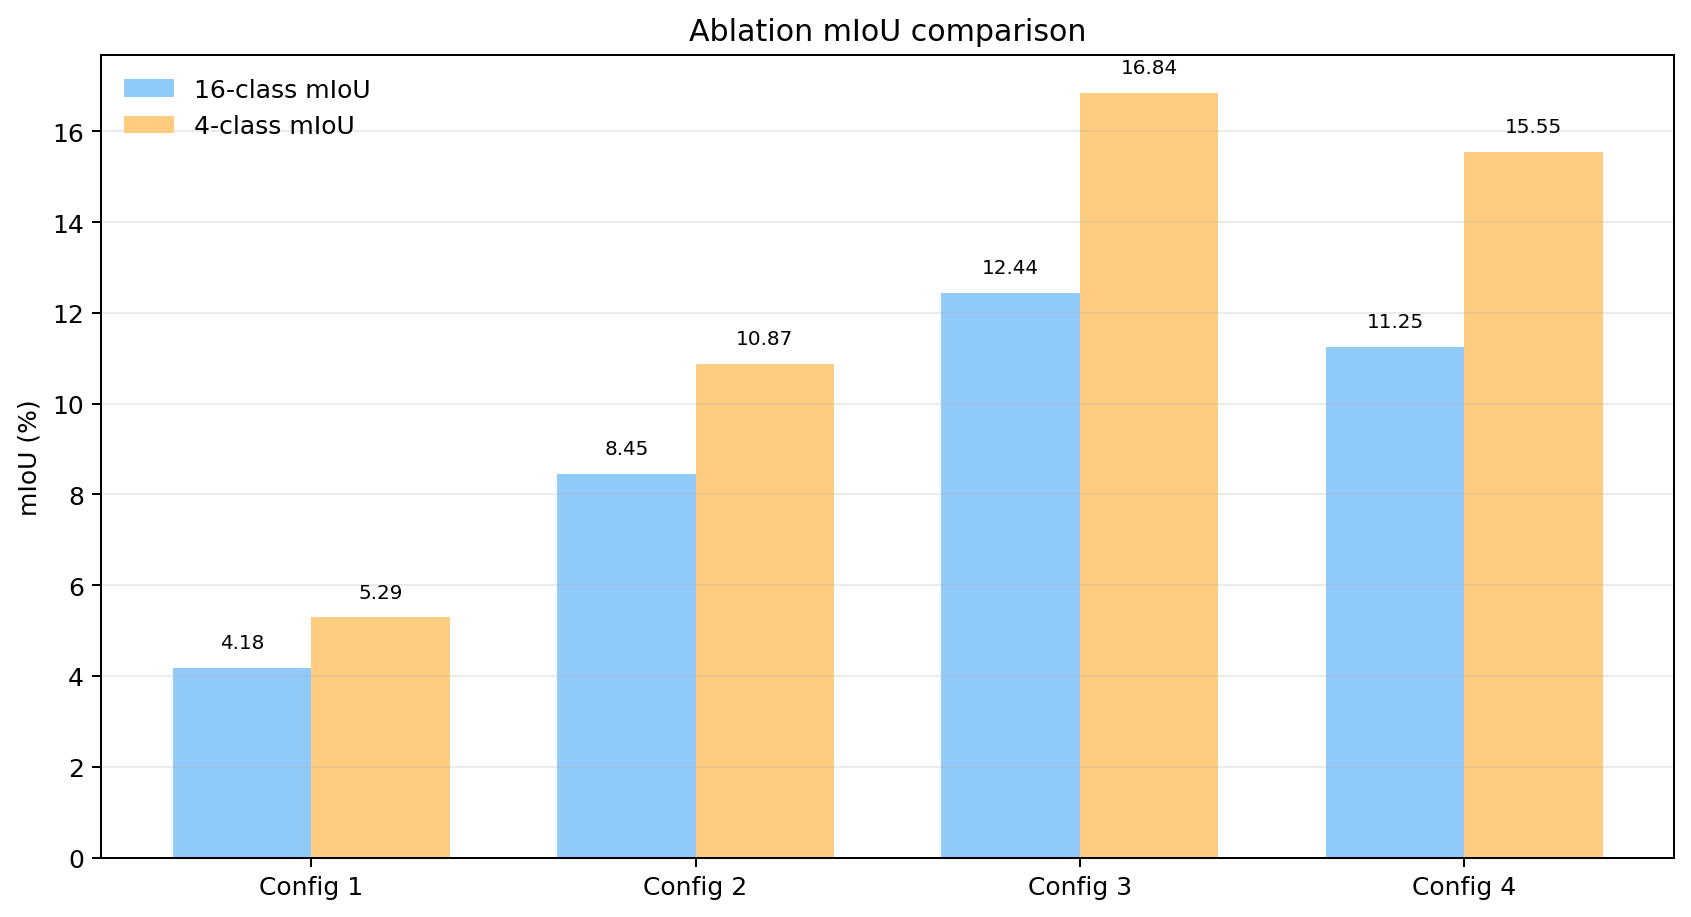
\includegraphics[width=0.9\textwidth]{figures/ablation_miou.png}
\caption{Quantitative comparison of ablation configurations in both evaluation spaces.}
\label{fig:miou-barplot}
\end{figure}

\begin{table}[h]
\centering
\caption{Per-superclass IoU (\%) in the remapped 4-class evaluation.}
\label{tab:ablation-remapped-classwise}
\begin{tabular}{|l|c|c|c|c|}
\hline
\textbf{Superclass} & \textbf{Config 1} & \textbf{Config 2} & \textbf{Config 3} & \textbf{Config 4} \\
\hline
Vegetation & 0.00 & 0.00 & 16.57 & 14.64 \\
Object & 1.25 & 0.75 & 2.62 & 0.90 \\
Ground & 0.25 & 11.61 & 9.70 & 10.43 \\
Structure & 19.67 & 31.12 & 38.48 & 36.23 \\
\hline
\end{tabular}
\end{table}

\section{Analysis of 16-Class Performance}
The original 16-class task remains challenging under severe domain mismatch. Baseline performance is low (4.18\% \ac{mIoU}), and predictions are unstable for sparse or absent categories.
\begin{itemize}
    \item \textbf{Baseline (Config 1):} The model collapses toward a few classes, with truck recall at 93.63\% but precision only 0.53\%, indicating severe overprediction. Vegetation \ac{IoU} is 0.00\%.
    \item \textbf{Zeroed intensity (Config 2):} Masking sensor-specific intensity improves 16-class \ac{mIoU} to 8.45\%, increases driveable-surface \ac{IoU} to 8.05\%, and raises manmade \ac{IoU} to 33.75\%.
    \item \textbf{Ring simulation (Config 3):} Simulated rings yield the strongest 16-class score (12.44\% \ac{mIoU}); vegetation \ac{IoU} recovers to 18.88\%, and manmade \ac{IoU} rises to 41.40\%.
    \item \textbf{Ring simulation (Config 4):} The stricter thin-ring setting remains effective (11.25\% \ac{mIoU}) but is slightly below Config 3, suggesting that overly aggressive thinning removes useful contextual geometry.
\end{itemize}

\section{Analysis of 4-Class Remapped Performance}
The 4-class remap offers a clearer view of scene-level understanding because it reduces sparsity and class-fragmentation effects.
\begin{itemize}
    \item \textbf{Baseline (Config 1):} The model overpredicts structure (19.67\% IoU) and fails on vegetation (0.00\% IoU), resulting in only 5.29\% \ac{mIoU}.
    \item \textbf{Config 2 (zeroed intensity):} Performance rises to 10.87\% \ac{mIoU}, with the strongest change in ground recognition (0.25\% to 11.61\% IoU).
    \item \textbf{Geometric adaptation (Configs 3 and 4):} Simulated ring structure gives the largest boost in vegetation and structure consistency; Config 3 reaches 16.84\%, while Config 4 reaches 15.55\%.
\end{itemize}
Across all configurations, the object superclass remains weak (below 3\% IoU), which indicates persistent viewpoint and scale mismatch for small or dynamic objects.

Overall, the 4-class analysis confirms that zero-shot adaptation is effective primarily for dominant scene components (ground, vegetation, structure), while sparse object categories remain an open challenge.

\begin{figure}[h]
\centering
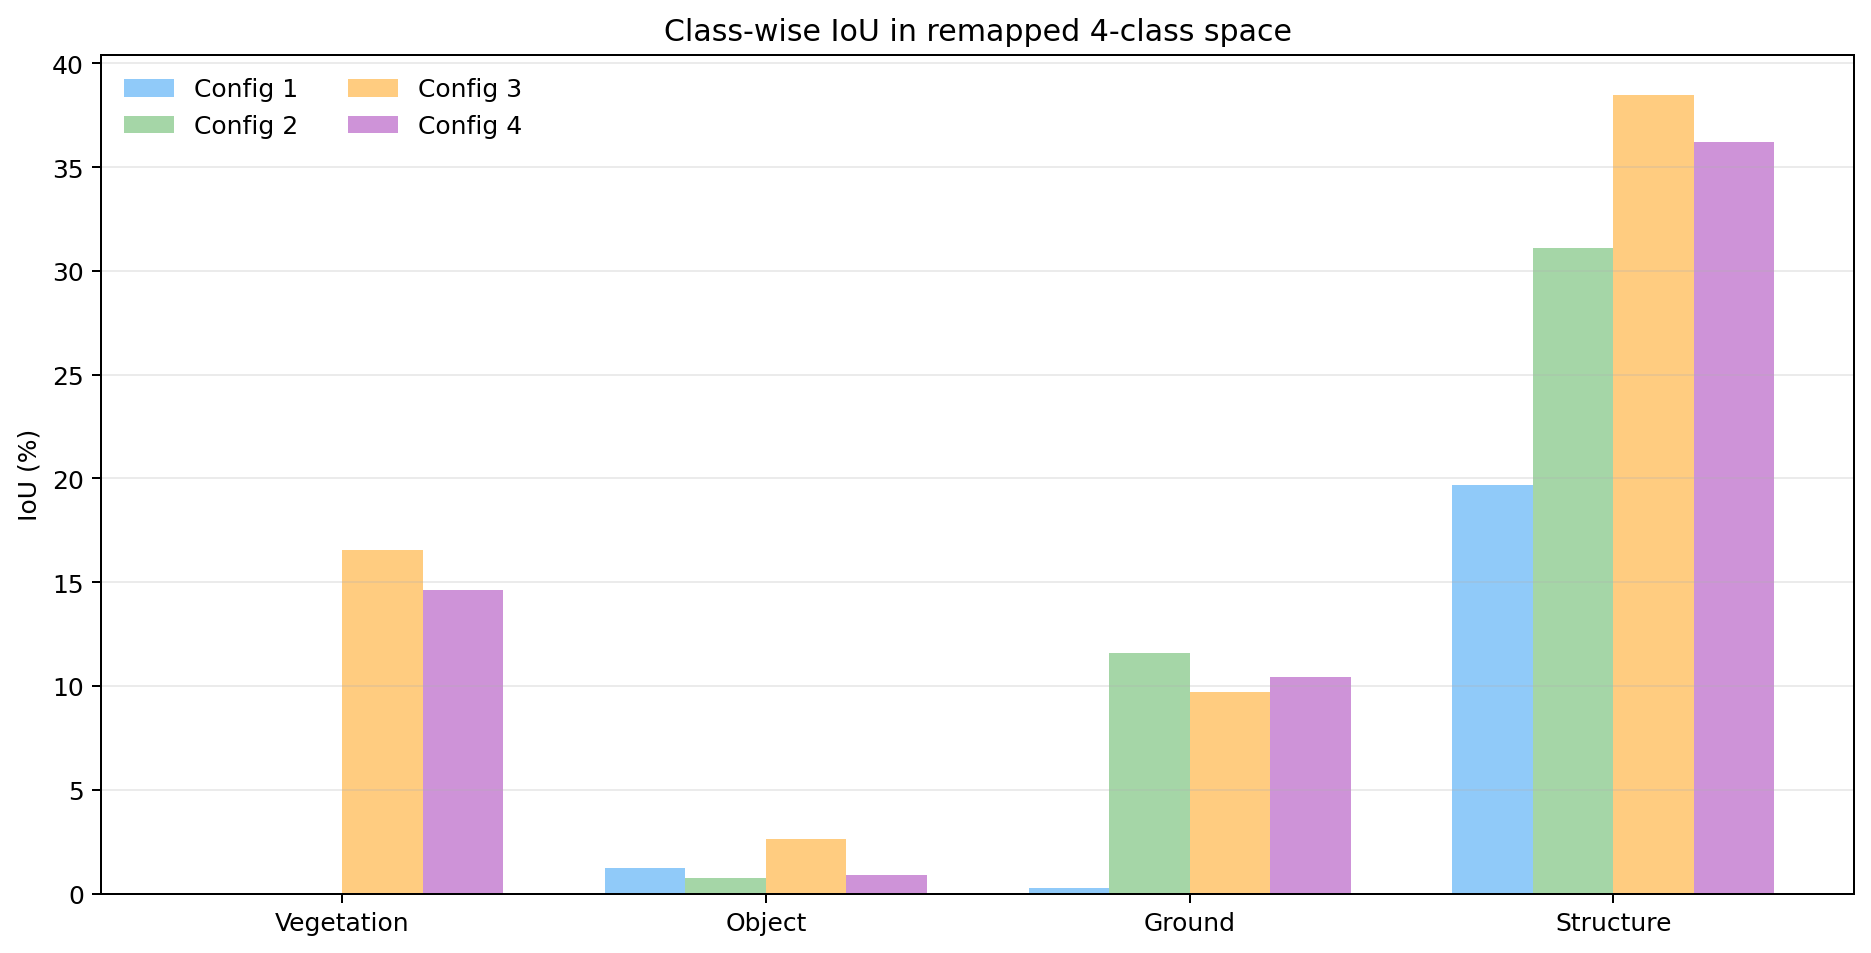
\includegraphics[width=0.9\textwidth]{figures/ablation_classwise_iou.png}
\caption{Class-wise performance trends in the remapped 4-class space.}
\label{fig:classwise-barplot}
\end{figure}

\section{Qualitative Assessment}
Qualitative inspection of full-scene outputs shows that adapted configurations better separate ground and vegetation than the baseline. Structural classes remain comparatively stable, while object-level classes (especially vehicles) are still inconsistent under viewpoint and density mismatch.

\begin{figure}[h]
\centering
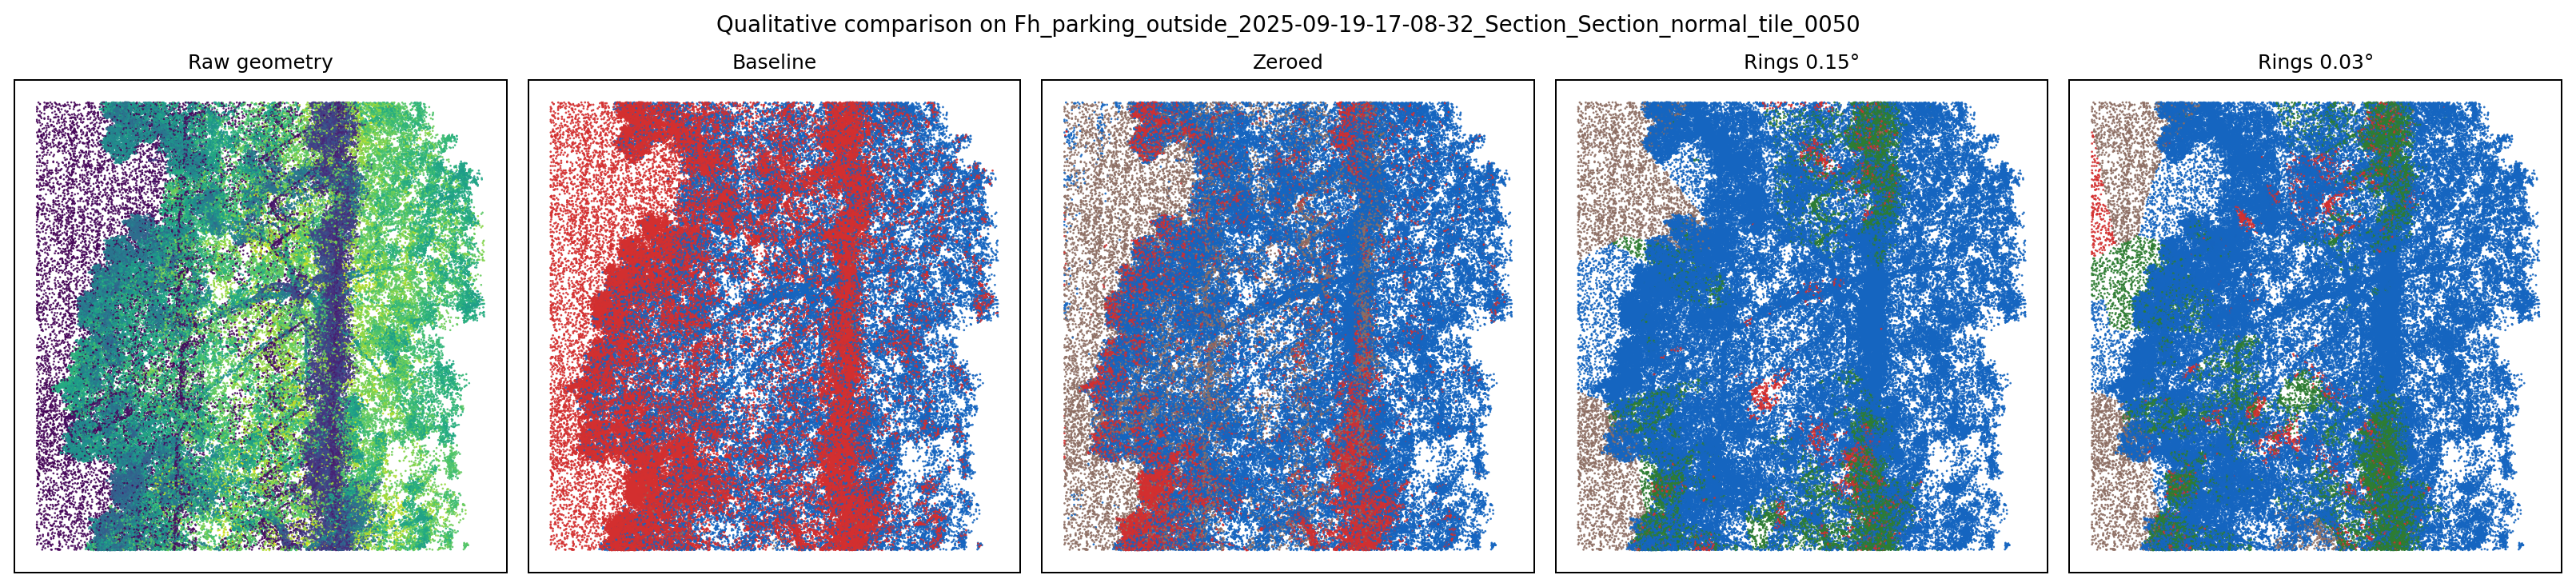
\includegraphics[width=0.95\textwidth]{figures/qualitative_comparison.png}
\caption{Qualitative comparison of segmentation outputs across ablation configurations.}
\label{fig:qualitative-comparison}
\end{figure}


\chapter{Discussion and Conclusion}
\section{Conclusions}
This report evaluated a zero-shot domain adaptation pipeline for transferring automotive 3D semantic segmentation models to high-density static LiDAR scans. Direct plug-and-play transfer fails, but targeted preprocessing substantially recovers performance. In particular, feature masking and ring-structure simulation raise 4-class \ac{mIoU} from 5.29\% to a best value of 16.84\% (Config 3), with the thin-ring variant achieving 15.55\% (Config 4).

The findings answer the research questions as follows: (i) useful scene-level outputs are achievable without retraining, (ii) geometric adaptation provides the largest incremental gain after intensity masking, and (iii) 4-class remapping significantly improves interpretability under domain mismatch.

\section{Practical Implications}
For urban-planning workflows, the adapted pipeline is already useful for rapid semantic structuring of large scenes, especially when the objective is to separate terrain, built structures, and vegetation. The method is also suitable as a preprocessing stage for downstream annotation, because it provides an informed initialization instead of starting from unlabeled geometry.

\section{Limitations}
Despite this gain, absolute accuracy remains modest, especially for object categories. The adaptation strategy is intentionally lossy: geometric downsampling discards high-resolution points, and viewpoint mismatch remains unresolved for small and dynamic objects.

Another limitation is that the evaluation uses a restricted label subset and a hand-labeled sample rather than a large benchmark-grade target dataset. Consequently, results should be interpreted as strong evidence of relative improvement, not as final production quality.

\section{Future Work}
Future work should prioritize supervised fine-tuning on a manually labeled subset of FJD Trion S1 data. Additional directions include \ac{UDA} methods (e.g., pseudo-labeling or adversarial alignment) and architecture comparisons for dense, unstructured point clouds.

A practical roadmap is:
\begin{enumerate}
    \item Curate a balanced target-domain label set with emphasis on sparse object classes.
    \item Fine-tune the existing \ac{PTv3} checkpoint using mixed source-target batches.
    \item Compare against architectures that do not assume ring-like sparsity as strongly.
    \item Quantify robustness across additional sites, seasons, and sensor settings.
\end{enumerate}

\section*{Recommended Visual Assets}
To strengthen the final report, the following images should be included at minimum:
\begin{itemize}
    \item Raw scene context (site-level overview) and one zoom-in of point density.
    \item Tiling visualization that shows overlap and boundary handling.
    \item Clear color legend for the 16-class and 4-class label spaces.
    \item One quantitative chart for mIoU progression and one for class-wise IoU.
    \item Side-by-side qualitative outputs (baseline vs. best adapted configuration).
\end{itemize}
% ==========================================
% 5. BACK MATTER (References & Appendix)
% ==========================================
\newpage
% Ensure you cite using IEEE format in your text, e.g., "As shown in \cite{example_source}..."
\printbibliography[heading=bibintoc, title={References}]

\newpage
\appendix
\chapter{Class Mapping and Experimental Details}
\label{app:class-mapping}

\begin{table}[h]
\centering
\caption{Mapping from 16 nuScenes-style classes to 4 project superclasses.}
\label{tab:class-map}
\begin{tabular}{|p{3.2cm}|p{10.3cm}|}
\hline
\textbf{4-Class Target} & \textbf{Mapped Source Classes} \\
\hline
Vegetation & vegetation \\
Object & car, truck, bus, trailer, motorcycle, bicycle, pedestrian, traffic cone, barrier, other object \\
Ground & driveable surface, sidewalk, terrain \\
Structure & manmade, building-like static structures \\
\hline
\end{tabular}
\end{table}

\begin{table}[h]
\centering
\caption{Ablation configuration summary.}
\label{tab:config-summary}
\begin{tabular}{|l|l|l|}
\hline
\textbf{Config} & \textbf{Feature Mode} & \textbf{Ring Tolerance} \\
\hline
1 & xyz+intensity & none \\
2 & zero & none \\
3 & zero & \SI{0.15}{\degree} \\
4 & zero & \SI{0.03}{\degree} \\
\hline
\end{tabular}
\end{table}

\begin{table}[h]
\centering
\caption{Reproducible command sequence used in all experiments.}
\label{tab:repro-commands}
\begin{tabular}{|p{3.2cm}|p{8.8cm}|}
\hline
\textbf{Stage} & \textbf{Command and Purpose} \\
\hline
Data tiling & \texttt{make tile} --- voxel subsampling and overlap-based tile generation \\
Inference & \texttt{make infer FEATURE\_MODE=<mode>} --- per-tile prediction with selected feature mode \\
Reconstruction & \texttt{make reconstruct} --- logit aggregation, softmax voting, and export of labeled \texttt{.las} outputs \\
\hline
\end{tabular}
\end{table}


% ==========================================
% 6. STATUTORY DECLARATION (Mandatory)
% ==========================================
\newpage
\chapter*{Declaration of Authorship}
\addcontentsline{toc}{chapter}{Declaration of Authorship}


I hereby declare that I have completed the present work independently and without the use of any aids other than those listed. Sentences and parts of sentences taken verbatim are marked as quotations; other adaptations with regard to statement and scope are identified with reference to the source. \par
\vspace{1cm}
The work has not yet been submitted to any examination authority in the same or similar form and has also not yet been published.\par
\vspace{3cm}

\noindent
\begin{tabular}{@{}p{6cm}p{2cm}p{6cm}@{}}
\hrulefill & & \hrulefill \\
Place, Date & & Signature
\end{tabular}

\end{document}